

% Gradient Info
  
\tikzset {_mi6touds3/.code = {\pgfsetadditionalshadetransform{ \pgftransformshift{\pgfpoint{0 bp } { 0 bp }  }  \pgftransformrotate{0 }  \pgftransformscale{2 }  }}}
\pgfdeclarehorizontalshading{_0gt4n9t5l}{150bp}{rgb(0bp)=(0.95,0.91,0.4);
rgb(37.5bp)=(0.95,0.91,0.4);
rgb(48.76041957310268bp)=(1,0.71,0.27);
rgb(100bp)=(1,0.71,0.27)}
\tikzset{every picture/.style={line width=0.75pt}} %set default line width to 0.75pt        

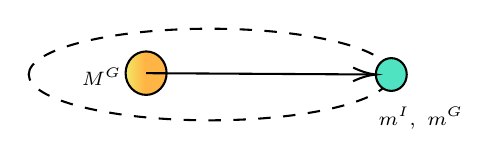
\begin{tikzpicture}[x=0.75pt,y=0.75pt,yscale=-1,xscale=1]
%uncomment if require: \path (0,120); %set diagram left start at 0, and has height of 120

%Shape: Ellipse [id:dp3388155288326359] 
\draw  [dash pattern={on 4.5pt off 4.5pt}] (242,51.07) .. controls (242,38.88) and (281.1,29) .. (329.34,29) .. controls (377.58,29) and (416.68,38.88) .. (416.68,51.07) .. controls (416.68,63.25) and (377.58,73.13) .. (329.34,73.13) .. controls (281.1,73.13) and (242,63.25) .. (242,51.07) -- cycle ;
%Shape: Ellipse [id:dp36789931790514396] 
\path  [shading=_0gt4n9t5l,_mi6touds3] (288.68,50.42) .. controls (288.68,44.64) and (293.1,39.95) .. (298.56,39.95) .. controls (304.01,39.95) and (308.43,44.64) .. (308.43,50.42) .. controls (308.43,56.2) and (304.01,60.88) .. (298.56,60.88) .. controls (293.1,60.88) and (288.68,56.2) .. (288.68,50.42) -- cycle ; % for fading 
 \draw   (288.68,50.42) .. controls (288.68,44.64) and (293.1,39.95) .. (298.56,39.95) .. controls (304.01,39.95) and (308.43,44.64) .. (308.43,50.42) .. controls (308.43,56.2) and (304.01,60.88) .. (298.56,60.88) .. controls (293.1,60.88) and (288.68,56.2) .. (288.68,50.42) -- cycle ; % for border 

%Shape: Ellipse [id:dp3599863720377383] 
\draw  [fill={rgb, 255:red, 80; green, 227; blue, 194 }  ,fill opacity=1 ] (409.24,51.07) .. controls (409.24,46.71) and (412.57,43.17) .. (416.68,43.17) .. controls (420.8,43.17) and (424.13,46.71) .. (424.13,51.07) .. controls (424.13,55.43) and (420.8,58.96) .. (416.68,58.96) .. controls (412.57,58.96) and (409.24,55.43) .. (409.24,51.07) -- cycle ;
%Straight Lines [id:da6952374372125172] 
\draw    (298.56,50.42) -- (407.24,51.05) ;
\draw [shift={(409.24,51.07)}, rotate = 180.34] [color={rgb, 255:red, 0; green, 0; blue, 0 }  ][line width=0.75]    (10.93,-3.29) .. controls (6.95,-1.4) and (3.31,-0.3) .. (0,0) .. controls (3.31,0.3) and (6.95,1.4) .. (10.93,3.29)   ;

% Text Node
\draw (409.13,65.47) node [anchor=north west][inner sep=0.75pt]  [font=\scriptsize]  {$m^{I} ,\ m^{G}$};
% Text Node
\draw (266.13,46.47) node [anchor=north west][inner sep=0.75pt]  [font=\scriptsize]  {$M^{G}$};


\end{tikzpicture}
